\section{Examination of solutions}
Several solutions have been proposed by Ethereum community (mostly from developers on GitHub) to address this attack. There would be some considerations for each solution that needs to be evaluated in term of compatibility with ERC20 standard and attack mitigation. We have examined technical aspects of each solution in the following sections.

\subsection{Enforcement by User Interface (UI)}
ERC20 standard recommends to set allowance to zero before any non-zero values and enforce approval processing check in UI instead of smart contract:
\begin{figure}[H]
	\centering
	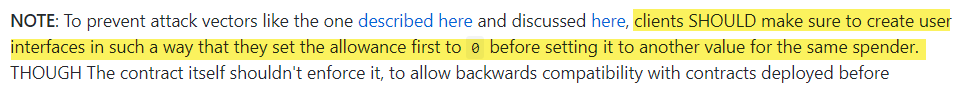
\includegraphics[width=1.0\linewidth]{figures/multiple_withdrawal_03.png}
	\caption{Recommendation of ERC20 standard to mitigate multiple withdrawal attack.}
\end{figure}
\noindent However, if Alice does not use UI and connects directly to the blockchain, there would be a good chance of impacting by this attack. Furthermore, as discussed on Github\cite{Ref14}, this approach is not sufficient and still allows Bob to transfer N+M tokens:
\begin{enumerate}
	\item Bob is allowed to transfer N Alice’s tokens.
	\item Alice publishes transaction that changes Bob’s allowance to 0.
	\item Bob front runs Alice’s transaction and transfers N Alice’s tokens (\textit{transferFrom} sets Bob’s allowance to 0).
	\item Alice’s transaction is mined and Bob’s allowance is set to 0 by \textit{approve} method. This is exactly what she would see if Bob would not transfer any tokens, so she has no reason to think that Bob actually used his allowance before it was revoked.
	\item Now Alice publishes a new transaction that changes Bob’s allowance to M.
	\item Alice’s second transaction is mined, Bob now is allowed to transfer M Alice’s tokens.
	\item Bob transfers M Alice’s tokens and in total N+M.\newline
\end{enumerate}
At step 3, Bob is able to transfer N tokens and consequently his allowance becomes 0. This is a legitimate transaction since Alice has already approved it. The issue occurs after Alice’s new transaction to set Bob's allowance to 0. In case of front-running by Bob, Alice needs to check Bob’s allowance for the second time before setting any new value. However, she will find out Bob’s allowance 0 in either case. In other words, she can not distinguish whether Bob’s allowance is set to 0 because of her transaction or Bob already transferred token on her behalf. Someone may point out that Alice notices this by checking \textit{Transfer} event logged by \textit{transferFrom} function. However, if Bob had transferred tokens to someone else (like Carol), then \textit{Transfer} event will not be linked to Bob, and, if Alice’s account is busy and many people are allowed to transfer from it, Alice may not be able to distinguish this transfer from a legitimate one performed by someone else. Overall, this solution does not prevent the attack while tries to follow ERC20 recommendations for setting Bob’s allowance to zero before any non-zero value. Additionally, There is no way to see from UI if setting Bob's allowance to 0 is processed before the subsequent non-zero approval \cite{Ref03}. This is because of current methods in Web3.js\footnote{JavaScript UI library for interacting with Ethereum blockchain} that do not support such checking\cite{Ref05}. Hence, enforcement should be considered at contract level not UI.\footnote{Interestingly, OpenZeppelin example implements a workaround in contract level that makes it inconsistent with the recommendations of ERC20.}

\subsection{Using Minimum viable token}
As suggested by\cite{Ref05}, we can boil down ERC20 standard to a very basic functionalities by implementing only essential methods. this will prevent effecting of the attack by skipping implementation of vulnerable functions. While removing \textit{approve} and \textit{transferFrom} functions prevent the attack, it makes the token partially-ERC20-compliant. Golem Network Token (GNT\footnote{https://etherscan.io/address/0xa74476443119A942dE498590Fe1f2454d7D4aC0d\#code}) is one of these examples since it does not implement the \textit{approve}, \textit{allowance} and \textit{transferFrom} functions. According to ERC20 specifications, these methods are not OPTIONAL and must be implemented. Moreover, ignoring them will cause failed function calls from standard smart contracts that expect to interact with these methods. Therefore, we would not consider this solution as a compatible fix although mitigates the attack.

\subsection{Approving trusted parties}
Approving token transfer to non-upgradable smart contracts can be considered safe. Because they do not contain any logic to take advantage of this vulnerability. However, upgradable smart contracts may add new logic to a new version that needs re-verification before approving token transfer. Similarly, approving token transfer to people that we trust could be considered as a mitigation plan. Nonetheless, this solution would have limited use cases and it could not be considered as a comprehensive mitigation for the attack.

\subsection{MiniMeToken solution}
MiniMeToken\cite{Ref15} also follows ERC20 recommendation by reducing allowance to zero before non-zero values. They added a line of code to the \textit{approve} method. The red clause allows setting approval to 0 and blue condition checks allowance of \textit{\_spender} to be 0 before setting to other values (i.e., If \textit{\_spender} allowance is 0 then allows non-zero values):
\begin{figure}[H]
	\centering
	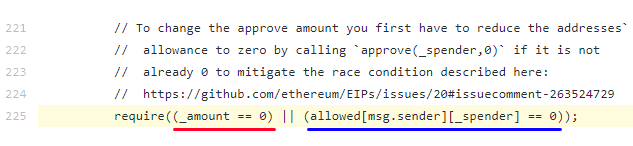
\includegraphics[width=1.0\linewidth]{figures/multiple_withdrawal_06.png}
	\caption{MiniMeToken suggestion for adding new codes to approve method.}
\end{figure}
\noindent Similar to "Enforcement by User Interface (UI)", this will not prevent Bob from transferring N+M tokens. Because Alice would not be able to distinguish whether N tokens have been already transferred or not. It is more clear in this scenario:
\begin{enumerate}
	\item Alice decides to set Bob’s allowance to 0.
	\item Bob front-runs Alice’s transaction and his allowance sets to 0 after transferring N tokens.
	\item Alice’s transaction is executed and sets Bob’s allowance to 0 (Red clause passes sanity check).
	\item Alice checks Bob’s allowance and she will find it 0, so, she can not determine whether this was because of her transaction or Bob already transferred N tokens.
	\item By considering that Bob has not been transferred any tokens, Alice allows Bob for transferring new M tokens.
	\item Bob would be able to transfer new approved tokens.
\end{enumerate}

\subsection{MonolithDAO solution}
MonolithDAO\cite{Ref12} Token suggests two additional functions for increasing or decreasing allowance. \textit{approve} function will also have an additional code to set allowance to zero before non-zero values. In this case, the default \textit{approve} function should be called when spender’s allowance is zero (No approval has been made). If spender’s allowance is non-zero, increase and decrease functions will be used:
\begin{figure}[H]
	\centering
	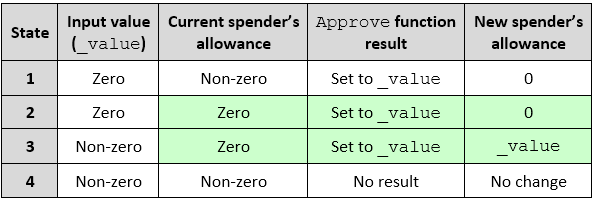
\includegraphics[width=1.0\linewidth]{figures/multiple_withdrawal_09.png}
	\caption{Functionality of \textit{approve} method with new added code in MonolithDAO token.}
\end{figure}
These two functions can address race condition and prevent allowance double-spend exploit:
\begin{enumerate}
	\item Alice allows Bob to transfer N tokens by calling \textit{approve(\_Bob, N)}. This will be executed by \textit{approve} function since current Bob’s allowance is 0.
	\item After a while, Alice decides to decrease Bob’s approval by M by running \textit{decreaseApproval(\_Bob, M)}.
	\item Bob notices Alice’s second transaction and front runs it by executing \textit{transferFrom(\_Alice, \_Bob, N)}.
	\item Bob’s transaction will be executed first and transfers N token to his account and the his allowance becomes 0 as result of this transfer.
	\item Alice’s transaction is mined after Bob’s transaction and tries to decrease Bob’s allowance by M. If Bob had already transferred more than M tokens, new Bob’s allowance becomes negative and it fails the transaction. So, the transaction does not change Bob’s remaining allowance and he would be able to transfer the rest (which is legitimate transfer since Alice has already approved it). If Bob had transferred less than M tokens, the new allowance will be applied and reduces Bob’s allowance by M.\newline
\end{enumerate}
\noindent Although these two new functions will prevent the attack, they have not been defined in the initial specifications of ERC20. Therefore, they can not be used by smart contracts that are already deployed on the Ethereum network since they will still use approve method for setting new allowance and not \textit{increaseApproval} or \textit{decreaseApproval}. Moreover, ERC20 specifications does not define any increase or decrease of allowance. It only defines new allowance. For example, if Alice has approved Bob for 100 tokens and wants to set it to 80, the new allowance should be 80 while using decrease methods will set it 20 (100 - 80 = 20). Comparatively, increase method will set new allowance to 180 while it has to set to 80 again. For these reasons, this solution would not be compatible with ERC20 standard and only is usable if approver or smart contract are aware of these supplementary methods.

\subsection{Alternate approval function}
Another suggestion\cite{Ref16} is to move security checks to another function like \textit{safeApprove} that sets allowance if it has not been already changed. By using this function, Alice uses the standard \textit{approve} function to set Bob’s allowance to 0 and for new approvals, she has to use \textit{safeApprove}. It takes the current expected approval amount as input parameter and calls \textit{approve} method if previous allowance is equal to current expected approval. So, Alice will have one step more and it is reading the current allowance and passing it to the new \textit{safeApprove} method. As mentioned in the last section, this approach is not backward compatible with already implemented smart contracts. The new \textit{safeApprove} method that is not defined in ERC20 standard and existing code would not be able to use this safety feature.

\subsection{Detecting token transfers}
As suggested by \cite{Ref17},a boolean variable is used to detect whether any tokens have been transferred or not. \textit{transferFrom} method sets a flag to true if tokens are transferred. \textit{approve} method checks the flag to be false before allowing new approvals (i.e., it checks if tokens have been used/transferred since the owner last allowance set). Moreover, it uses a new data structure for keeping track of used/transferred tokens. This approach could prevent race condition as described below:
\begin{enumerate}
	\item Alice runs \textit{approve(\_Bob, N)} to allow Bob for transferring N tokens.
	\item Since Bob’s initial allowance is 0 and used flag is false, then sanity check passes and Bob’s allowance is set to N.
	\item Alice decides to set Bob’s allowance to 0 by executing \textit{approve(\_Bob, 0)}.
	\item Bob front-runs Alice’s transaction and transfers N tokens. Then, his used flag turns to \textit{true}.
	\item Alice’s transaction is mined and passes sanity check (because \textit{\_value == 0}).
	\item Bob’s allowance is set to 0 while used flag is still \textit{true}.
	\item Alice changes Bob’s allowance to M by executing \textit{approve(\_Bob, M)}.
	\item Since Bob already transferred number of tokens, used flag is \textit{true} and it fails the transaction.
	\item Bob’s allowance remains as N and he could transfer only N tokens.\newline
\end{enumerate}
\noindent Although this approach mitigates the attack, it prevents any further legitimate approvals as well. Considering a scenario that Alice rightfully wants to increase Bob’s allowance from N to M (two non-zero values). If Bob had already transferred number of tokens (even 1 token), Alice would not be able to change his approval. Because used flag is \textit{true} now and does not allow changing allowance to any non-zero values. Even setting the allowance to 0, does not flip used flag and keeps Bob’s allowance locked down. In fact, the code needs a line like \textit{allowed[\_from][msg.sender].used = false;} in \textit{approve} method. But it will cause another problem. After setting allowance to 0, used flag becomes \textit{false} and allows non-zero values event if tokens have been already transferred. In other words, it resembles the initial values of allowance similar when nothing is transferred. Therefore, it makes attack mitigation functionality ineffective. In short, this approach can not satisfy both legitimate and non-legitimate scenarios and violets ERC20 standard that says:
\begin{figure}[H]
	\centering
	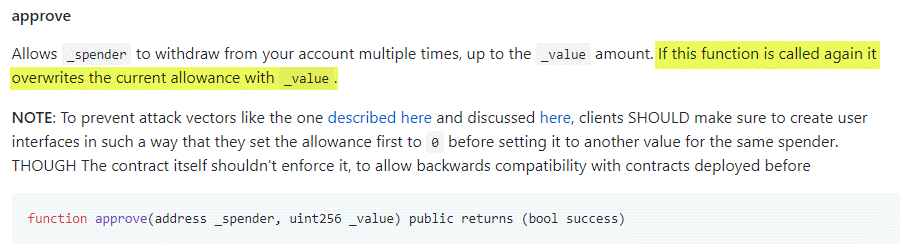
\includegraphics[width=1.0\linewidth]{figures/multiple_withdrawal_28.png}
	\caption{ERC20 approve method constraint.}
\end{figure}
\noindent Nevertheless, this solution is a step forward by introducing the need for a new variable to track transferred tokens.

\subsection{Keeping track of remaining tokens}
Inspired by by the previous solution, \cite{Ref18} keeping track of remaining tokens instead of detecting transferred tokens. It uses modified version of data structure that used in the previous solution for storing residual tokens:
\begin{figure}[H]
	\centering
	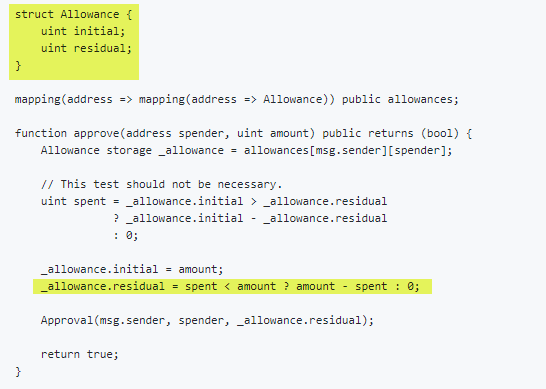
\includegraphics[width=1.0\linewidth]{figures/multiple_withdrawal_29.png}
	\caption{Keeping track of remaining tokens.}
\end{figure}
At first, it seems that this solution is a sustainable way to mitigate the attack by setting approval to zero before non-zero values. However, the highlighted code resembles the situation that we explained in "Enforcement by User Interface (UI)":
\begin{enumerate}
	\item Bob’s allowance is initially zero (\textit{allowances[\_Alice][\_Bob].initial=0}, \textit{allowances[msg.sender][spender].residual=0}).
	\item Alice allows Bob to transfer N tokens (\textit{allowances[\_Alice][\_Bob].initial=N}, \textit{allowances[\_Alice][\_Bob].residual=N}).
	\item Alice decides to change Bob’s allowance to M and has to set it to zero before any non-zero values.
	\item Bob noticed Alice’s transaction for setting his allowance to zero and transfers N tokens in advance. transferFrom sets his allowance (residual) to zero consequently (\textit{allowances[\_Alice][\_Bob].residual=0}).
	\item Alice’s transaction is mined and sets \textit{allowances[\_Alice][\_Bob].initial=0} and \textit{allowances[msg.sender][spender].residual=0} (Similar to step 1). This is like that no token has been transferred. So, Alice would not be able to distinguish whether any token have been transferred or not.
	\item Alice approves Bob for spending new M tokens.
	\item Bob is able to transfer new M tokes in addition to initial N tokens.\newline
\end{enumerate}
Someone may think of using \textit{Transfer} event to detect transferred tokens or checking approver balance to see any transferred tokens. As explained in "Enforcement by User Interface (UI)", using \textit{Transfer} event is not sufficient in case of transferring tokens to a third party. Checking approver balance also would not be an accurate way if the contract is busy and there are lot of transfers. So, it would be difficult for the approver to detect legitimate from non-legitimate tokens transfers.

\subsection{Changing ERC20 API}
\cite{Ref03} advised to change ERC20 approve method to compare current allowance of spender and sets it to new value if it has not already been transferred. This allows atomic compare and set of spender allowance to make the attack impossible. So, it will need new overloaded approve method with three parameters:
\begin{figure}[H]
	\centering
	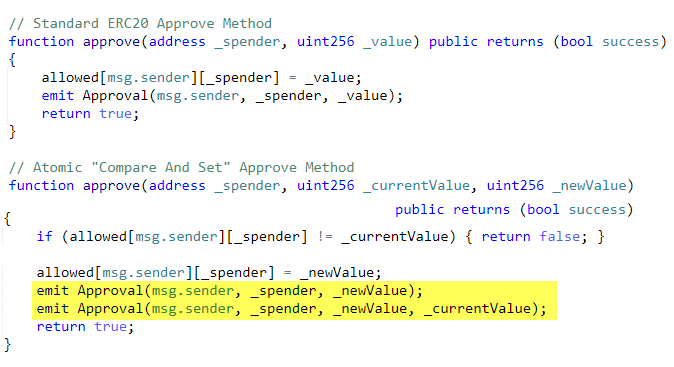
\includegraphics[width=1.0\linewidth]{figures/multiple_withdrawal_12.png}
	\caption{Suggested ERC20 API Change for approve method.}
\end{figure}
In order to use this new method, smart contracts have to update their codes to provide three parameters instead of current two, otherwise any \textit{approve} call will throw an exception. Moreover, one more call is required to read current allowance value and pass it to the new approve method. New events need to be added to ERC20 specification to log an approval events with four arguments. For backward compatibility reasons, both three-arguments and new four-arguments events have to be logged. All of these changes makes this token contract incompatible with deployed smart contracts and software wallets. Hence, it could not be considered as viable solution.

\subsection{New token standards}
After recognition of this security vulnerability, new standards like ERC233 \footnote{https://github.com/Dexaran/ERC223-token-standard} and ERC721\footnote{https://github.com/ethereum/EIPs/blob/master/EIPS/eip-721.md} were introduced to address the issue in addition to improving current functionality of ERC20 standard. They changed approval model and fixed some drawbacks which need to be addressed in ERC20 as well (i.e., handle incoming transactions through a receiver contract, lost of funds in case of calling transfer instead of transferFrom, etc). Nevertheless, migration from ERC20 to ERC223/ERC721 would not be convenient and all deployed tokens needs to be redeployed. This also means update of any trading platform listing ERC20 tokens. The goal here is to find a backward compatible solution instead of changing current ERC20 standard or migrating tokens to new standards. Despite expanded features and improved security properties of new standards, we would not consider them as target solutions.